\begin{frame}[fragile]{$\Sigma^\ast$}
%\alert{Für \Sigma = \{a,b\}}:
\begin{figure}
    \centering
    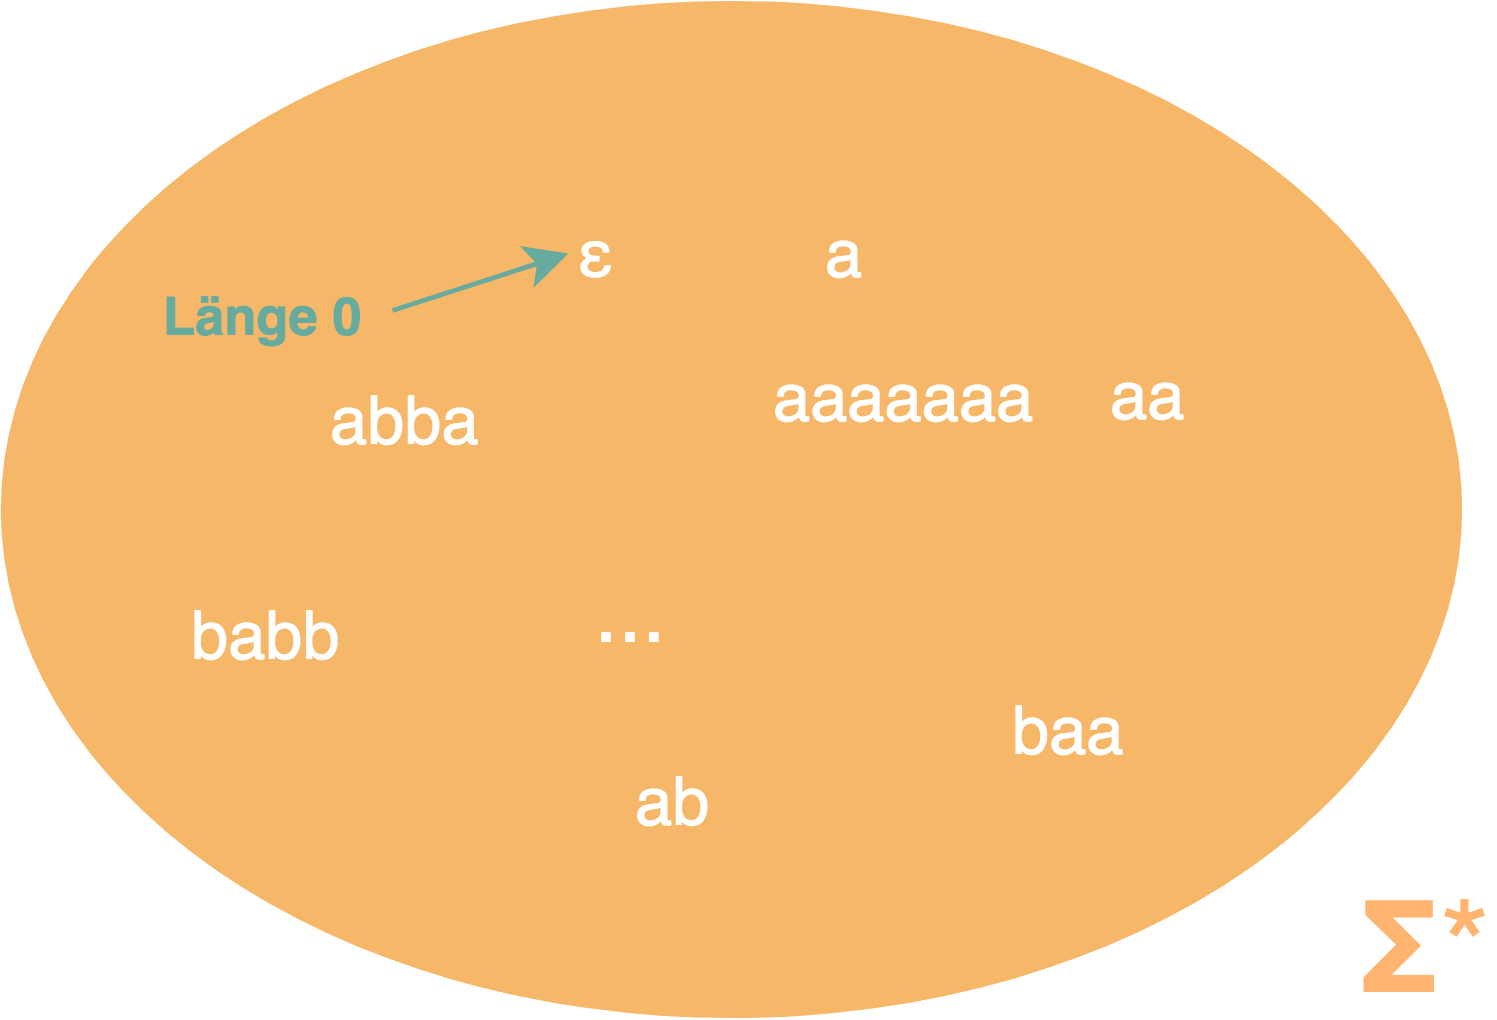
\includegraphics[width=0.7\textwidth]{../figures/SigmaSternEpsilon.png}
    \caption{Menge von allen Kombinationen der Elemente von $\Sigma$ heißt $\Sigma^\ast$}
\end{figure}
\end{frame}

\begin{frame}[fragile]{$\Sigma^\ast$}
    %\metroset{block=fill}
    \begin{exampleblock}{Das heißt\dots}
    Sei $\Sigma = \{a,b\}$ unser \alert{Alphabet}.\\
    Wir beschreiben die Menge, die alle Möglichkeiten enthält Elemente aus $\Sigma$ zu \emph{konkatenieren} mit $\Sigma^\ast=\{\emptyWord,a,b,aa,ab,ba,bb,aba,\dots\}$.
    \end{exampleblock}\pause
    
    \begin{alertblock}{Achtung}
    $M^\ast$ über einer beliebigen Menge $M$ enthält immer das leere Wort $\emptyWord$!\\
    Sogar wenn $M = \{\} = \emptyset$.\\
    
    \end{alertblock}
\end{frame}

{\setbeamercolor{palette primary}{bg=ExColor}
\begin{frame}[fragile]{Denkpause}
    \begin{alertblock}{Aufgaben}
    Nenne jeweils 5 der kürzesten Elemente aus $\alert{\Sigma^{*}}$ für die folgenden Alphabete $\alert\Sigma$:
    \end{alertblock}
    
    \metroset{block=fill}
    \begin{block}{Normal}
        \begin{itemize}
            \item $\Sigma = \{a\}$
            \item $\Sigma = \{0, 1, 2, 3, 4, 5, 6, 7, 8, 9\}$
        \end{itemize}
    \end{block}
    \metroset{block=fill}
    \begin{block}{Etwas schwerer}
        \begin{itemize}
            \item $\Sigma$ = \{0, x, Biber\}
            \item $\Sigma$ = \{\Smiley, \Frowny\}
        \end{itemize}
    \end{block}
\end{frame}
}

{\setbeamercolor{palette primary}{bg=ExColor}
\begin{frame}{Lösungen}
    Mögliche Lösungen sind \dots
  \begin{itemize}[<+- | alert@+>]
        \item $\emptyWord, a, aa, aaa, aaaa \in \{a\}^{*}$
        \item $\emptyWord, 0, 1, 2, 3\in \{0,1,2,3,4,5,6,7,8,9\}^{*}$
        \item $\emptyWord, 0, x, Biber, xBiber \in \{0, x, Biber\}^{*}$
        \item $\emptyWord$, \Smiley, \Frowny, \Smiley\Smiley, \Smiley\Frowny$\; \in \{$\Smiley, \Frowny$\}^{*}$
    \end{itemize}
\end{frame}
}

\begin{frame}[fragile]{Alphabete und $\Sigma^{*}$}
\begin{alertblock}{Verständnisabfrage}
    Denke kurz über folgende Aufgabe nach...
    \end{alertblock}
    
    \metroset{block=fill}
    \begin{block}{Schwer}
        Welche Wörter sind in $M^{*}$ enthalten, wenn $M = \emptyset$ gilt?
    \end{block}
\end{frame}

{\setbeamercolor{palette primary}{bg=ExColor}
\begin{frame}{Lösungen}
  \begin{itemize}
        \item In $M^{*} = \{$ $ \}^{*}$ ist \textbf{nur} das leere Wort $\emptyWord$ enthalten.
    \end{itemize}
\end{frame}
}

\begin{frame}[fragile]{Sprachen}
\begin{figure}
    \centering
    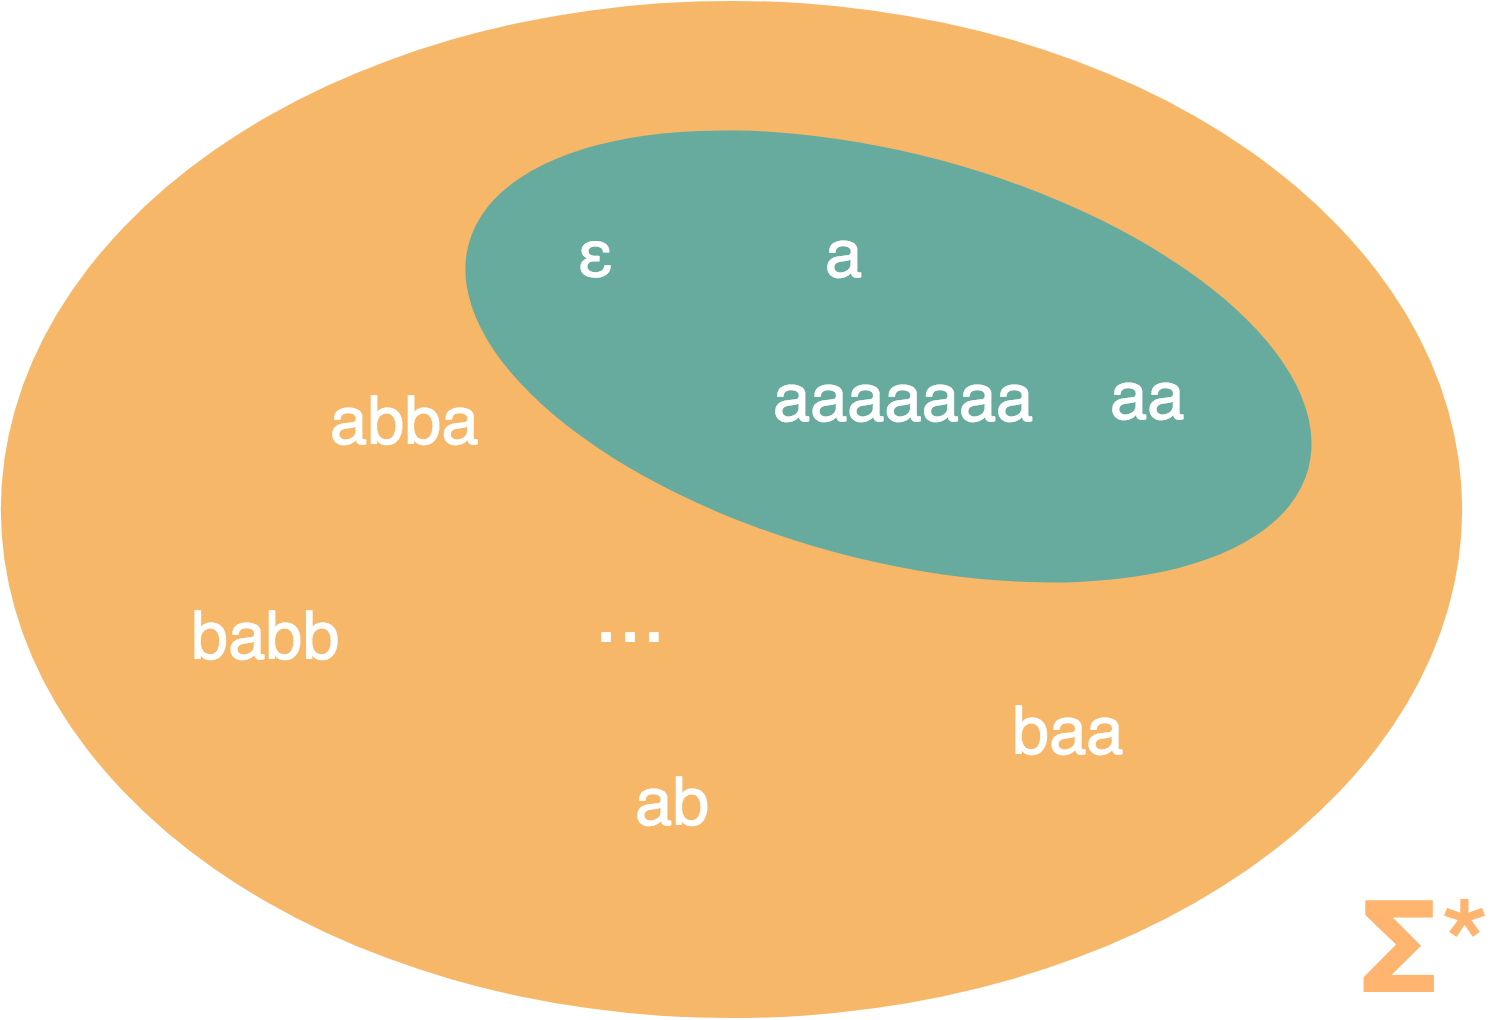
\includegraphics[width=0.7\textwidth]{../figures/MysterySprache.png}
    \caption{Teilmengen unserer Obermenge nennen wir Sprachen}
    \label{fig:my_label}
\end{figure}
\end{frame}

\begin{frame}[fragile]{Sprachen beschreiben}
\begin{figure}
    \centering
    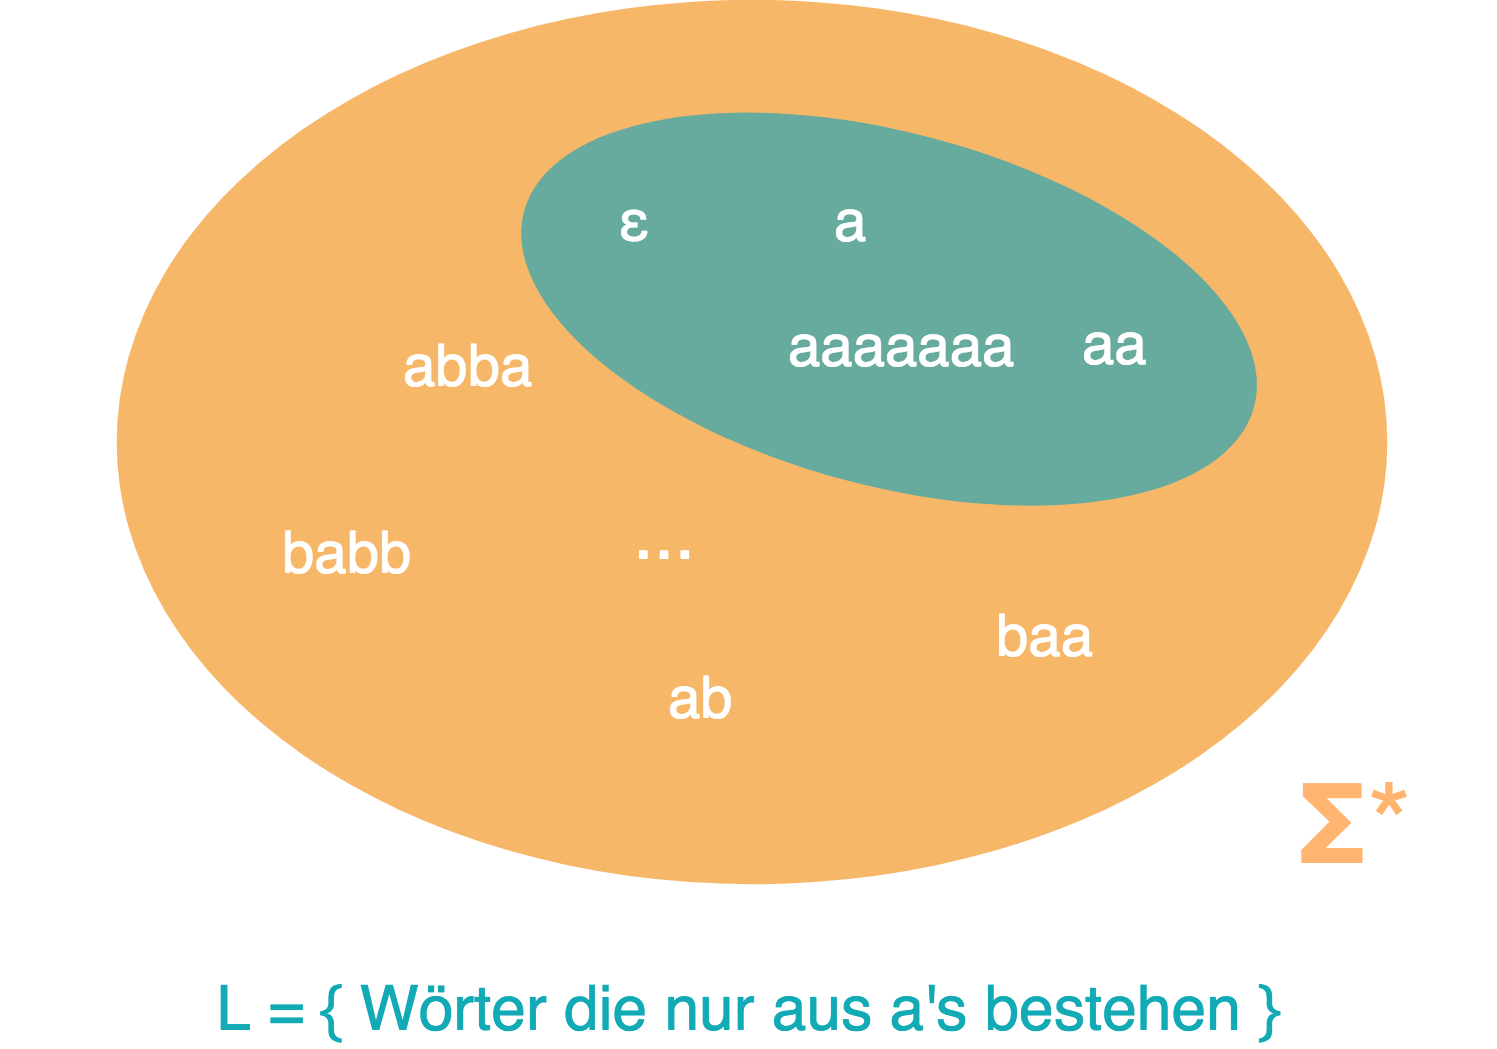
\includegraphics[width=0.7\textwidth]{../figures/SprachReveal.png}
    \caption{Manche Sprachen können wir mit Regeln beschreiben}
    \label{fig:my_label}
\end{figure}
\end{frame}

\begin{frame}[fragile]{Sprachen beschreiben}
    \metroset{block=fill}
    \begin{exampleblock}{Beispiele für Sprachen in Mengenschreibweise}
    \begin{itemize}
        \item $L_1 = \{a^n\;|\;n\in\mathbb{N}\}$
        \item $L_2 = \{a^n\;|\;n \equiv 0 \bmod 2, n\in\mathbb{N}\}$
        \item $L_3 = \{uv\;|\;u\in\{a,b\}^\ast,\;v\in\{a\}\}$
        \item $L_4 = \{w\;|\;|w|_a = 3\}$
    \end{itemize}
    \end{exampleblock}
    Was soll das alles? Mehr dazu nach der Pause :)
\end{frame}
